\section{Metamodel for  existing notations and their interoperabilities to SACM}
\label{sec:mapping}
SACM is designed to support existing safety notations such as GSN and CAE. In previous sections, we briefly demonstrated the semantics of SACM elements by comparing them with GSN notations. In this section, we provide a GSN metamodel and a CAE metamodel that are compliant to SACM. We also discuss the interoperability from GSN and CAE to SACM.

\subsection{The GSN Metamodel and the inteoperability from GSN to SACM}
As previously discussed, SACM provides a richer set of features comparing to GSN, which includes the ability to standardise evidential and informational artifacts in the models, standardising controlled grammar and terminologies, as well as modular organisation and integration of artifacts and terminologies. In general, creating a metamodel for GSN is a simple task, for there are only several concepts that GSN captures. However, we think it is more ideal to create the GSN metamodel by extending SACM elements, so that not only the GSN metamodel can inherit features provided by SACM, but also making the interoperability from GSN to SACM easier. 
\begin{figure}
	\centering
	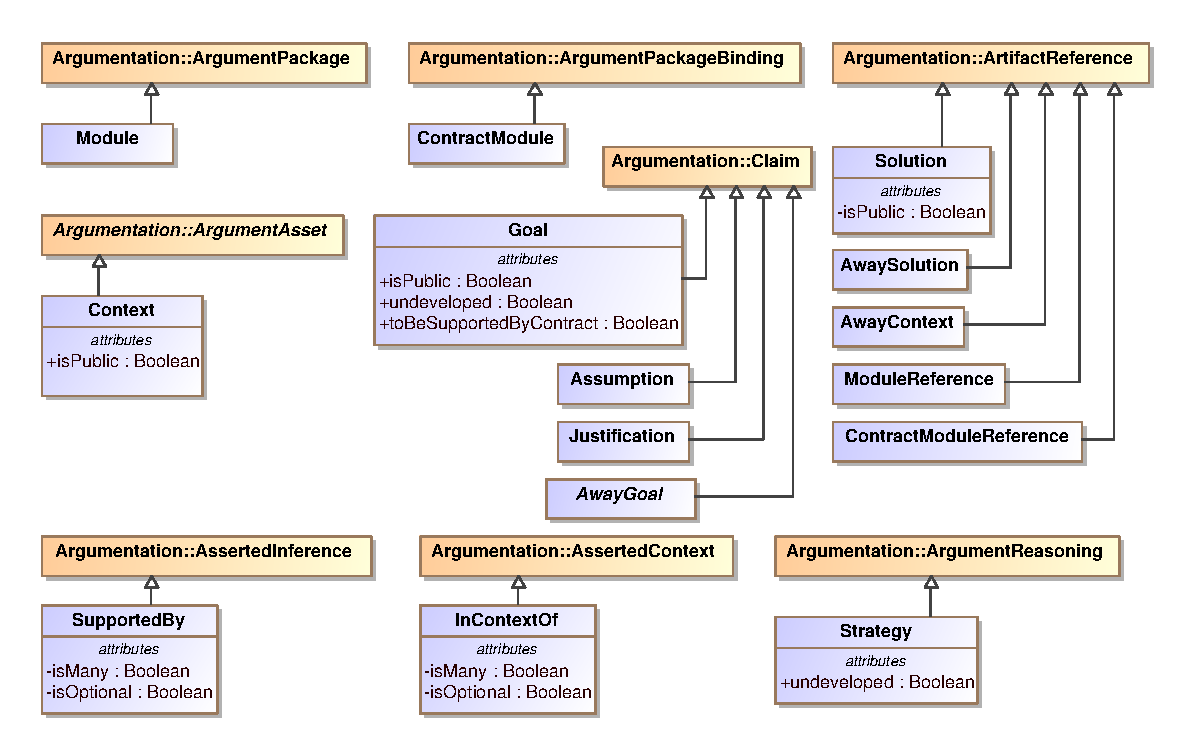
\includegraphics[width=1\linewidth]{GSN.eps}
	\caption{SACM compliant GSN metamodel.}
	\label{fig:gsnMetamodel}
\end{figure}

Our version of the GSN metamodel is shown in Figure~\ref{fig:gsnMetamodel}. In GSN, argumentations are organised in \textit{Module}s, which is made as a sub-type of \textit{ArgumentPackage} in SACM; \textit{ContractMoudle} are essentially contracts that binds \textit{Module}s together, thus it is a sub-type of \textit{ArgumentPackageBinding}. 

Elements \textit{Goal}, \textit{Assumption}, \textit{Justification} and \textit{AwayGoal} are made sub-types of \textit{Claim} in SACM. A \textit{Goal} can be \textit{uninstantiated}, which basically means it is abstract, this is captured by the \textit{+isAbstract} feature in SACM's \textit{SACMElement} class. A \textit{Goal} can be \textit{public}, which is deprecated in SACM, a \textit{Goal} can also be \textit{undeveloped} and \textit{toBeSupportedByContract}, which are captured individually. 

Elements \textit{Solution}, \textit{AwaySolution}, \textit{AwayContext}, \textit{ModuleReference} and \textit{ContractModuleReference} are sub-types of \textit{ArtifactReference} in SACM as they refer to artefacts that contain information they represent. \textit{Context} is a slightly complicated concept, as it can either be a statement stating the context of a \textit{Claim}, or it can refer to contextual information stored in an artefact. Thus, \textit{Context} is made a sub-type of \textit{ArgumentAsset}. 

\textit{SupportedBy} is made a sub-type of \textit{AssertedInference} and \textit{InContextOf} is made a sub-type of \textit{AssertedContext}. \textit{Strategy} is made a sub-type of \textit{ArgumentReasoning} for it explains the intention of an \textit{AssertedRelationship}.

The way that the GSN metamodel is created makes it inherently capable of modelling artefacts and terminologies due to the fact that the GSN metamodel also inherits the the \textit{Base}, \textit{AssuranceCase}, \textit{Artifact} and \textit{Terminology} packages. Our vision is that such GSN metamodel is able to create goal structures, and link evidential and contextual information from the goal structures to their supporting materials, modelling using the \textit{Artifact} and \textit{Terminology} packages. 

\begin{algorithm}[ht!]
	{
		\fontsize{9}{10}
		\selectfont
		\SetAlgoLined\DontPrintSemicolon
		\SetKwFunction{getUpperLevelSupportedBy}{strategy}
		\SetKwFunction{getLowerLevelSupportedBy}{strategy}
		\SetKwFunction{createModelElement}{createModelElement}
		\SetKwFunction{getCachedModelElement}{getCachedModelElement}
		\SetKwFunction{setFeatureValue}{setFeatureValue}
		\SetKwFunction{setAttributeValue}{setAttributeValue}
		\SetKwFunction{handleObjectAttributes}{handleObjectAttributes}
		\SetKwFunction{handleFeature}{handleFeature}
		
		\SetKwFunction{shouldHandleFeature}{shouldHandleFeature}
		
		\SetKwProg{Procedure}{Procedure}{}{}
		
		\Let strategy = \textit{Strategy} to be transformed;\\
		\Let argumentReasoning = new \textit{ArgumentReasoning};\\
		\Let incomingSupportedBy = the incoming \textit{SupportedBy} to \textit{strategy};\\
		\Let outgoingSupportedBy = all outgoing \textit{SupportedBy}s from \textit{strategy};\\
		argumentReasoning.name = strategy.name.equivalent();\\
		argumentReasoning.description = strategy.description.equivalent();\\
		\If {strategy.uninstantiated == true} {
			argumentReasoning.isAbstract = true;
		}
		\Let supportedByToSolution = all \textit{SupportedBy}s from \textit{outgoingSupportedBy} \\
		that connects to a \textit{Solution};\\
		\If{supportedByToSolution is not empty}{
			\Let assertedEvidence = new \textit{AssertedEvidence};\\
			assertedEvidence.target = incomingSupportedBy.source;\\
			\For{supportedBy in supportedByToSolution}{
				assertedEvidence.source.add(supportedBy.target);\\
			}
		}
		\Let supportedByToGoal = all \textit{SupportedBy}s from \textit{outgoingSupportedBy} \\
		that connects to a \textit{Goal};\\
		\If{supportedByToGoal is not empty}{
			\Let assertedInference = new \textit{AssertedInference};\\
			assertedInference.target = assertedInference.source;\\
			\For{supportedBy in supportedByToGoal}{
				assertedInference.source.add(supportedBy.target);\\
			}
		}
	}
	\
	\caption{Transforming Strategy into ArgumentReasoning}
	\label{alg:s2ar}
\end{algorithm}

To enable interoperability from GSN to SACM, we provide a model-to-model transformation\footnote{Available at: \url{https://github.com/wrwei/MDERE/blob/master/technical}} defined using the Epsilon Transformation Language\cite{kolovos2008epsilon}. Most part of the transformation is straight forward - instances of the GSN elements are transformed into instances of the SACM elements that the GSN elements extend. There is one exception: the transformation from \textit{Strategy} to \textit{ArgumentReasoning}. As discussed in Section~\ref{sec:relationships}, an \textit{ArgumentReasoning} is associated to an \textit{AssertedRelationship}, but in GSN, a \textit{Strategy} acts as a node in a goal structure. This requires that analysis to be performed during the transformation, which is shown in Algorithm~\ref{alg:s2ar}.

\subsection{The CAE metamodel and the interoprability from CAE to SACM}
Claims, Arguments and Evidence (CAE) \cite{cae} is another widely used notation to construct safety arguments. Concepts in CAE are similar to those in GSN. There has not been an official metamodel defined for CAE. Thus, we provide our own version of CAE that extends SACM, shown in Figure~\ref{fig:caeMetamodel}.
\begin{figure}
	\centering
	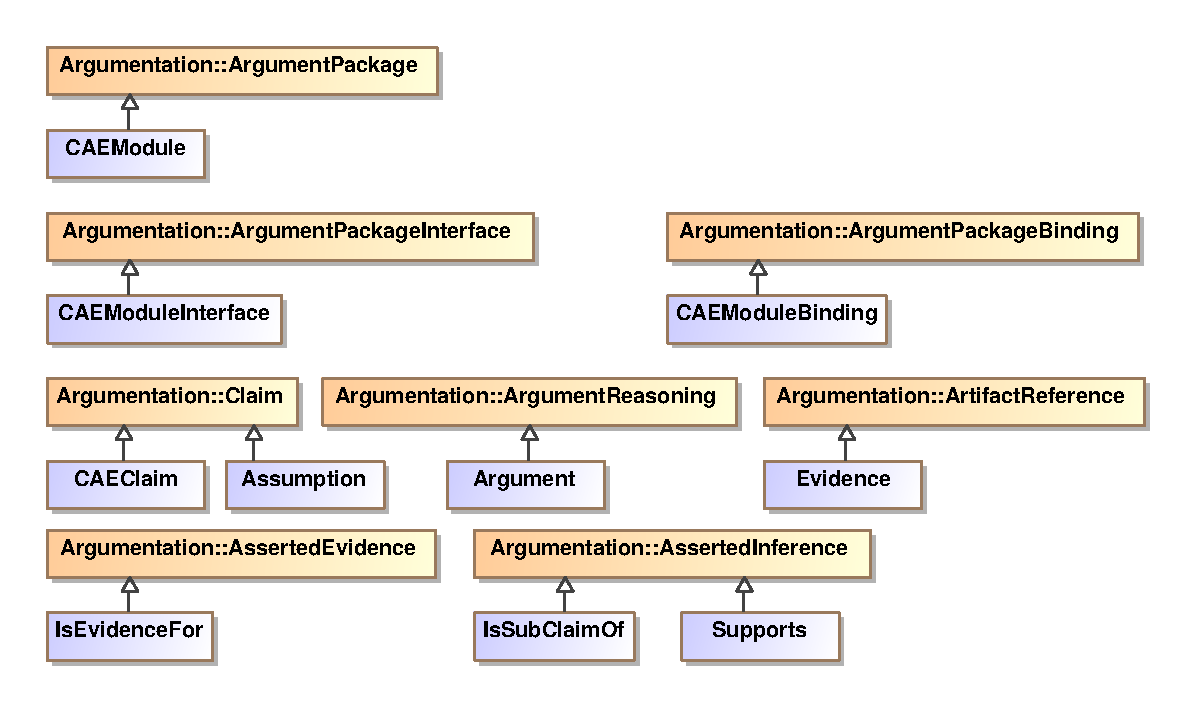
\includegraphics[width=1\linewidth]{CAE.eps}
	\caption{SACM compliant CAE metamodel.}
	\label{fig:caeMetamodel}
\end{figure}

In CAE, there is a notion of \textit{Claim}, thus it is not necessary to duplicate \textit{Claim} in SACM. The \textit{Argument} elements in CAE provides a description of the argument approach, which is functionally equivalent to \textit{ArgumentReasoning}, thus it is made a sub-type of \textit{ArgumentReasoning}. \textit{Evidence} is made a sub-type of \textit{ArtifactReference} because it is a reference to evidential materials. In CAE, there is a notion of \textit{Assumption}, which is made a sub-type of \textit{Claim}. 

In CAE, there are three types of relationships, the \textit{IsEvidenceFor} connects \textit{Evidence} with \textit{Claim}s, thus is made a sub-type of \textit{AssertedEvidence}; the \textit{IsSubClaimOf} relationship connects sub-\textit{Claim}s to \textit{Claim} and is made a sub-type of \textit{AssertedInference}; the \textit{Supports} relationship connects \textit{Argument}s to \textit{Claim} and is also made a sub-type of \textit{AssertedInference}. Since there is no notion of modules in CAE, the argumentation is contained in \textit{ArgumentPackage}s inherited from SACM.

The transformation from CAE to SACM is similar to the transformation from GSN to SACM (which is also implemented in Epsilon Transformation Language), with the same issue that a model analysis is needed when transforming \textit{Argument} to \textit{ArgumentReasoning}. The detailed transformation is made publicly available\footnote{Available at: \url{https://github.com/wrwei/MDERE/blob/master/technical}}.



